\section{Accessing hardware devices}

\subsection{Kernel drivers}

\begin{frame}{Typical software stack for hardware access}
  \begin{columns}
    \column{0.6\textwidth}
    From the bottom to the top:
    \begin{itemize}
    \item A {\em bus controller driver} in the kernel drives an I2C,
      SPI, USB, PCI controller
    \item A {\em bus subsystem} provides an API for drivers to access
      a particular type of bus: I2C, SPI, PCI, USB, etc.
    \item A {\em device driver} in the kernel drives a particular
      device connected to a given bus
    \item A {\em driver subsystem} exposes features of certain class
      of devices, through a standard {\em kernel/user-space interface}
    \item An application can access the device through this standard {\em
        kernel/user-space interface} either directly or through a
      library.
    \end{itemize}
    \column{0.4\textwidth}
    \begin{center}
      \includegraphics[height=0.7\textheight]{slides/sysdev-hw-devices/kernel-driver-stack.pdf}
    \end{center}
  \end{columns}
\end{frame}

\begin{frame}{Stack illustrated with a GPIO expander}
  \begin{center}
    \includegraphics[height=0.8\textheight]{slides/sysdev-hw-devices/kernel-driver-stack-gpio-i2c.pdf}
  \end{center}
\end{frame}

\begin{frame}{Standardized user-space interface}
  \begin{itemize}
  \item Strong advantage of kernel drivers: they expose a standard
    {\em kernel to user-space interface}
  \item All devices of the same class (e.g GPIO controllers) will
    expose the same {\em kernel to user-space interface}
  \item Applications don't have to know the details of the GPIO
    controller, they just need to know the standard user-space
    interface valid for all GPIO controllers
  \item Applications can use existing open-source libraries that
    leverage this standard user-space interface
  \item Such kernel drivers can also be used internally inside the
    kernel, for example if one driver needs to control a GPIO directly
    (reset signal, interrupt signal, etc.)
  \end{itemize}
\end{frame}

\begin{frame}{Numerous kernel subsystems for device classes}
  \begin{columns}
    \column{0.5\textwidth}
    \begin{itemize}
    \item Networking stack for Ethernet, WiFi, CAN, 802.15.4, etc.
    \item GPIO
    \item Video4Linux for camera, video encoders/decoders
    \item DRM for display controllers, GPU
    \item ALSA for audio
    \item IIO for ADC, DAC, gyroscopes, sensors, and more
    \item MTD for flash memory
    \item PWM
    \end{itemize}
    \column{0.5\textwidth}
    \begin{itemize}
    \item Input for keyboard, mouse, touchscreen, joystick
    \item Watchdog
    \item RTC for real-time clocks
    \item remoteproc for auxilliary processors
    \item crypto for cryptographic accelerators
    \item hwmon for hardware monitoring sensors
    \item block layer for block storage
    \end{itemize}
  \end{columns}
  \begin{center}
    and many more
  \end{center}
\end{frame}

\begin{frame}{Accessing devices directly from user-space}
  \begin{itemize}
  \item Even though device drivers in the kernel are preferred, it is
    also possible to access devices directly from user-space
  \item Especially useful for very specific devices that do not fit in
    any existing kernel subsystems
  \item The kernel provides the following mechanisms, depending on the
    bus:
    \begin{itemize}
    \item I2C: \href{https://docs.kernel.org/i2c/dev-interface.html}{i2c-dev}
    \item SPI: \href{https://docs.kernel.org/spi/spidev.html}{spidev}
    \item Memory-mapped: \href{https://docs.kernel.org/driver-api/uio-howto.html}{UIO}
    \item USB: \code{/dev/bus/usb}, through \href{https://libusb.info/}{libusb}
    \item PCI: \href{https://docs.kernel.org/PCI/sysfs-pci.html}{sysfs entries for PCI}
    \end{itemize}
  \end{itemize}
\end{frame}

\begin{frame}{Accessing devices directly from user-space: GPIO example}
  \begin{columns}
    \column{0.3\textwidth} {\small This diagram shows what's not
      recommended to do $\rightarrow$ for a GPIO controller, a kernel driver
      is preferred}
    \column{0.7\textwidth}
    \begin{center}
      \includegraphics[height=0.8\textheight]{slides/sysdev-hw-devices/kernel-driver-stack-gpio-i2c-direct-userspace.pdf}\\
    \end{center}
  \end{columns}
\end{frame}

\begin{frame}{What can go wrong with a user-space driver?}
  \begin{itemize}
  \item You write your GPIO driver in user-space: other kernel drivers
    cannot use GPIOs from this GPIO controller
    \begin{itemize}
    \item Other devices that use GPIO signals from this controller for reset, interrupt, etc. cannot control/configure those signals
    \end{itemize}
  \item You write your touchscreen driver in user-space: the standard
    Linux graphics stack components cannot use your touchscreen
  \item You write your network driver in user-space
    \begin{itemize}
    \item You can probably send/receive packets
    \item But you cannot leverage the Linux kernel networking stack
      for IP, TCP, UDP, etc.
    \item And none of the Linux networking applications can use your
      network device
    \end{itemize}
  \end{itemize}
\end{frame}

\begin{frame}{Upstream drivers vs. out-of-tree drivers}
  \begin{itemize}
  \item The {\em upstream} Linux kernel contains thousands of drivers
    \begin{itemize}
    \item This is the best place to look for drivers
    \item Drivers have been reviewed and approved by the community
    \item They comply with standard interfaces
    \end{itemize}
  \item Vendor kernels often include additional drivers, directly in
    the kernel tree
  \item Device vendors sometimes also provide {\em out of tree
      drivers}
    \begin{itemize}
    \item Their source code is provided separately from the Linux
      kernel tree
    \item Quality is often dubious
    \item Compatibility issues when updating to newer kernel releases
    \item Not always use standard user-space interfaces
    \item Example: \url{https://github.com/lwfinger/rtl8723ds}
    \item Avoid them when possible!
    \end{itemize}
  \end{itemize}
\end{frame}

\begin{frame}{Finding Linux kernel drivers}
  \begin{itemize}
  \item \code{grep} in the Linux kernel tree is your {\em best friend}
    \begin{itemize}
    \item For I2C, SPI and memory-mapped devices, matching of the
      driver is done based on the device name $\rightarrow$ {\em grep}
      for variants of the device name and vendor
    \item For USB, PCI, matching is done either on the vendor
      ID/product ID, or the class $\rightarrow$ {\em grep} for these
    \end{itemize}
  \item Driver file names are sometimes named in a ``generic'' way,
    not necessarily reflecting all devices they support.
    \begin{itemize}
    \item Example: \kfile{drivers/gpio/gpio-pca953x.c} supports much
      more than just PCA953x. See the
      \href{https://elixir.bootlin.com/linux/v5.19/source/drivers/gpio/gpio-pca953x.c\#L1221}{full
        list of devices} supported by this driver
    \end{itemize}
  \end{itemize}
\end{frame}

\begin{frame}[fragile]{Finding Linux kernel drivers: an example}
  \begin{itemize}
  \item You have a
    \href{https://www.maximintegrated.com/en/products/interface/controllers-expanders/MAX7313.html}{Maxim
      Integrated MAX7313} GPIO expander on I2C
  \item Search in the Linux kernel
    \begin{block}{git grep -i max7313}
      {\tiny
\begin{verbatim}
drivers/gpio/gpio-pca953x.c:    { "max7313", 16 | PCA953X_TYPE | PCA_INT, },
drivers/gpio/gpio-pca953x.c:    { .compatible = "maxim,max7313", .data = OF_953X(16, PCA_INT), },
\end{verbatim}
      }
    \end{block}
  \item \kfile{drivers/gpio/gpio-pca953x.c} seems to support it
  \item Read \kfile{drivers/gpio/Makefile} to learn which kernel
    configuration option enables this driver
    \begin{block}{\kfile{drivers/gpio/Makefile}}
      {\tiny
\begin{verbatim}
obj-$(CONFIG_GPIO_PCA953X)              += gpio-pca953x.o
\end{verbatim}
      }
    \end{block}
  \item Conclusion: you need to enable \kconfig{CONFIG_GPIO_PCA953X} in
    your kernel configuration
  \end{itemize}
\end{frame}

\subsection{User-space interfaces to drivers}

\begin{frame}{User-space interfaces for hardware devices}

  For a high-level perspective: three main interfaces to access
  hardware devices exposed by the Linux kernel

  \begin{itemize}
  \item Device nodes in \code{/dev}
  \item Entries in the {\em sysfs} filesystem
  \item Network sockets and related APIs
  \end{itemize}
\end{frame}

\begin{frame}{Devices in {\em /dev/}}
  \begin{itemize}
  \item One of the kernel important roles is to {\bf allow applications
      to access hardware devices}
  \item In the Linux kernel, most devices are presented to user space
    applications through two different abstractions
    \begin{itemize}
    \item {\bf Character} device
    \item {\bf Block} device
    \end{itemize}
  \item Internally, the kernel identifies each device by a triplet of
    information
    \begin{itemize}
    \item {\bf Type} (character or block)
    \item {\bf Major} (typically the category of device)
    \item {\bf Minor} (typically the identifier of the device)
    \end{itemize}
  \item See \kfile{Documentation/admin-guide/devices.txt} for the
    official list of reserved type/major/minor numbers.
  \end{itemize}
\end{frame}

\begin{frame}{Block vs. character devices}
  \begin{itemize}
  \item Block devices
    \begin{itemize}
    \item A device composed of fixed-sized blocks, that can be read
      and written to store data
    \item Used for hard disks, USB keys, SD cards, etc.
    \end{itemize}
  \item Character devices
    \begin{itemize}
    \item Originally, an infinite stream of bytes, with no beginning,
      no end, no size. The pure example: a serial port.
    \item Used for serial ports, terminals, but also sound cards,
      video acquisition devices, frame buffers
    \item Most of the devices that are not block devices are
      represented as character devices by the Linux kernel
    \end{itemize}
  \end{itemize}
\end{frame}

\begin{frame}{Devices: everything is a file}
  \begin{itemize}
  \item A very important UNIX design decision was to represent most
    {\em system objects} as files
  \item It allows applications to manipulate all {\em system objects} with
    the normal file API (\code{open}, \code{read}, \code{write},
    \code{close}, etc.)
  \item So, devices had to be represented as files to the applications
  \item This is done through a special artifact called a {\bf device
      file}
  \item It is a special type of file, that associates a file name
    visible to user space applications to the triplet {\em (type,
      major, minor)} that the kernel understands
  \item All {\em device files} are by convention stored in the
    \code{/dev} directory
  \end{itemize}
\end{frame}

\begin{frame}[fragile]{Device files examples}

Example of device files in a Linux system

\small
\begin{verbatim}
$ ls -l /dev/ttyS0 /dev/tty1 /dev/sda /dev/sda1 /dev/sda2 /dev/sdc1 /dev/zero
brw-rw---- 1 root disk    8,  0 2011-05-27 08:56 /dev/sda
brw-rw---- 1 root disk    8,  1 2011-05-27 08:56 /dev/sda1
brw-rw---- 1 root disk    8,  2 2011-05-27 08:56 /dev/sda2
brw-rw---- 1 root disk    8, 32 2011-05-27 08:56 /dev/sdc
crw------- 1 root root    4,  1 2011-05-27 08:57 /dev/tty1
crw-rw---- 1 root dialout 4, 64 2011-05-27 08:56 /dev/ttyS0
crw-rw-rw- 1 root root    1,  5 2011-05-27 08:56 /dev/zero
\end{verbatim}
\normalsize

Example C code that uses the usual file API to write data to a serial port

\small
\begin{minted}{c}
int fd;
fd = open("/dev/ttyS0", O_RDWR);
write(fd, "Hello", 5);
close(fd);
\end{minted}
\end{frame}

\begin{frame}{Creating device files}
  \begin{itemize}
    \item Before Linux 2.6.32, on basic Linux systems,
    the device files had to be created manually using the
    \code{mknod} command
    \begin{itemize}
    \item \code{mknod /dev/<device> [c|b] major minor}
    \item Needs root privileges
    \item Coherency between device files and devices handled by the
      kernel was left to the system developer
    \end{itemize}
  \item The \code{devtmpfs} virtual filesystem can be mounted on
    \code{/dev} $\rightarrow$ the kernel automatically creates/removes
    device files
    \begin{itemize}
    \item \kconfig{CONFIG_DEVTMPFS_MOUNT} $\rightarrow$ asks the
      kernel to mount {\em devtmpfs} automatically at boot time
      (except when booting on an initramfs).
    \end{itemize}
  \end{itemize}
\end{frame}

\begin{frame}{Better handling of device files: {\em udev} and {\em mdev}}
  \begin{itemize}
  \item {\em devtmpfs} is great, but its capabilities are limited, so
    complementary solutions exist
  \item {\bf udev}
    \begin{itemize}
    \item daemon that receives events from the kernel about devices
      appearing/disappearing
    \item can create/remove device files (but that's done by
      {\em devtmpfs} now), adjust permission/ownership,
      load kernel modules automatically, create symbolic links to
      devices
    \item according to rules files in \code{/lib/udev/rules.d} and
      \code{/etc/udev/rules.d}
    \item used in almost all desktop Linux distributions
    \item \url{https://en.wikipedia.org/wiki/Udev}
    \end{itemize}
  \item {\bf mdev}
    \begin{itemize}
    \item lightweight implementation of {\em udev}, part of Busybox
    \item \url{https://wiki.gentoo.org/wiki/Mdev}
    \end{itemize}
  \end{itemize}
\end{frame}

\begin{frame}{Examples of user-space interface in {\tt /dev}}
  \begin{itemize}
  \item Serial-ports: \code{/dev/ttyS*}, \code{/dev/ttyUSB*},
    \code{/dev/ttyACM*}, etc.
  \item GPIO controllers (modern interface): \code{/dev/gpiochipX}
  \item Block storage devices: \code{/dev/sd*}, \code{/dev/mmcblk*}, \code{/dev/nvme*}
  \item Flash storage devices: \code{/dev/mtd*}
  \item Display controllers and GPUs: \code{/dev/dri/*}
  \item Audio devices: \code{/dev/snd/*}
  \item Camera devices: \code{/dev/video*}
  \item Watchdog devices: \code{/dev/watchdog*}
  \item Input devices: \code{/dev/input/*}
  \item and many more...
  \end{itemize}
\end{frame}

\begin{frame}{{\em sysfs} filesystem}
  \begin{itemize}
  \item \code{block/}, symlinks to all block devices, in
    \code{/sys/devices}
  \item \code{bus/}, one sub-folder by type of bus
  \item \code{class/}, one sub-folder per class (category of devices):
    input, leds, pwm, etc.
  \item \code{dev/}
    \begin{itemize}
    \item \code{block/}, one symlink per block device, named after
      major/minor
    \item \code{char/}, one symlink per character device, named after
      major/minor
    \end{itemize}
  \item \code{devices/}, all devices in the system, organized in a
    slightly chaotic way, see \href{https://lwn.net/Articles/646617/}{this article}
  \item \code{firmware/}, representation of firmware data
    \begin{itemize}
    \item \code{devicetree/}, directory and file representation of
      Device Tree nodes and properties
    \end{itemize}
  \item \code{fs/}, properties related to filesystem drivers
  \item \code{kernel/}, properties related to various kernel subsystems
  \item \code{module/}, properties about kernel modules
  \item \code{power/}, power-management related properties
  \end{itemize}
\end{frame}

\begin{frame}[fragile]{{\em sysfs} filesystem example}
  \begin{itemize}
  \item \code{/sys/bus/i2c/drivers}: all device drivers for devices
    connected on I2C busses
    \begin{block}{}
      {\tiny
\begin{verbatim}
[...]
edt_ft5x06
stpmic1
[...]
\end{verbatim}
      }
    \end{block}

  \item \code{/sys/bus/i2c/devices}: all devices in the system
    connected to I2C busses
    \begin{block}{}
      {\tiny
\begin{verbatim}
0-002a -> ../../../devices/platform/soc/40012000.i2c/i2c-0/0-002a
0-0039 -> ../../../devices/platform/soc/40012000.i2c/i2c-0/0-0039
0-004a -> ../../../devices/platform/soc/40012000.i2c/i2c-0/0-004a
1-0028 -> ../../../devices/platform/soc/5c002000.i2c/i2c-1/1-0028
1-0033 -> ../../../devices/platform/soc/5c002000.i2c/i2c-1/1-0033
i2c-0 -> ../../../devices/platform/soc/40012000.i2c/i2c-0
i2c-1 -> ../../../devices/platform/soc/5c002000.i2c/i2c-1
i2c-2 -> ../../../devices/platform/soc/40012000.i2c/i2c-0/i2c-2
\end{verbatim}
      }
    \end{block}
  \end{itemize}
\end{frame}

\begin{frame}[fragile]{{\em sysfs} filesystem example}
  \begin{block}{/sys/bus/i2c/devices/0-002a/}
    {\tiny
\begin{verbatim}
lrwxrwxrwx    driver -> ../../../../../../bus/i2c/drivers/edt_ft5x06
-rw-r--r--    gain
drwxr-xr-x    input
-r--r--r--    modalias
-r--r--r--    name
lrwxrwxrwx    of_node -> ../../../../../../firmware/devicetree/base/soc/i2c@40012000/touchscreen@2a
-rw-r--r--    offset
-rw-r--r--    offset_x
-rw-r--r--    offset_y
drwxr-xr-x    power
-rw-r--r--    report_rate
lrwxrwxrwx    subsystem -> ../../../../../../bus/i2c
-rw-r--r--    threshold
-rw-r--r--    uevent
\end{verbatim}
    }
  \end{block}

  \begin{itemize}
  \item \code{driver}, symlink to the driver directory in \code{/sys/bus/i2c/drivers}
  \item \code{of_node}, symlink to the directory for the Device Tree
    node describing this device
  \end{itemize}
\end{frame}

\begin{frame}{Example of driver interfaces in {\em sysfs}}
  \begin{itemize}
  \item All devices are visible in {\em sysfs}, whether they have an
    interface in \code{/dev} or not
    \begin{itemize}
    \item Usually \code{/dev} is to access the device
    \item \code{/sys} is more about properties of the devices
    \end{itemize}
  \item However, some devices only have a {\em sysfs} interface
    \begin{itemize}
    \item LED: \code{/sys/class/leds}, see \href{https://docs.kernel.org/leds/leds-class.html}{documentation}
    \item PWM: \code{/sys/class/pwm}, see \href{https://docs.kernel.org/driver-api/pwm.html\#using-pwms-with-the-sysfs-interface}{documentation}
    \item IIO: \code{/sys/class/iio}, see \href{https://docs.kernel.org/driver-api/iio/index.html}{documentation}
    \item etc.
    \end{itemize}
  \end{itemize}
\end{frame}

\begin{frame}{Accessing GPIOs}
  A class of devices worth mentioning is GPIOs ({\em General Purpose Input Output})
  \begin{itemize}
  \item The GPIOs can be accessed through a legacy interface in
        \code{/sys/class/gpios}
    \begin{itemize}
       \item You will find many instructions on the Internet about how
	     to drive GPIOs through this interface.
       \item However, this interface is deprecated and has multiple
             shortcomings:
             \begin{itemize}
		\item GPIOs remain exported if the process using them crashes
		\item Need to compute the GPIO numbers, such numbers are not stable
	     \end{itemize}
    \end{itemize}
  \item A new interface recommended: \href{https://git.kernel.org/pub/scm/libs/libgpiod/libgpiod.git/}{libgpiod}
    \begin{itemize}
	\item Based on \code{/dev/gpiochipx} character devices
        \item Implementing advanced features not possible with the legacy interface
	\item Of course, this is a C library
        \item But it also provides command line utilities:
              \code{gpiodetect}, \code{gpioset}, \code{gpioget}...
	\item The only constraint is to cross-compile them for your target
	      (the legacy interface could be used without any additional software).
    \end{itemize}
  \end{itemize}
\end{frame}

\begin{frame}{Other virtual filesystems}

  \begin{itemize}

  \item {\em debugfs}
    \begin{itemize}
    \item Conventionally mounted in \code{/sys/kernel/debug}
    \item Contains lots of debug information from the kernel,
      including device related
    \item \code{/sys/kernel/debug/pinctrl} for pin-mux debugging,
      \code{/sys/kernel/debug/gpio} for GPIO debugging,
      \code{/sys/kernel/debug/pwm} for PWM debugging, etc.
    \item \url{https://www.kernel.org/doc/html/latest/filesystems/debugfs.html}
    \end{itemize}
  \item {\em configfs}
    \begin{itemize}
    \item Conventionally mounted in \code{/sys/kernel/config}
    \item Allows to manage configuration of advanced kernel mechanisms
    \item Example: configuration of USB gadget functionalities
    \item \kfile{Documentation/filesystems/configfs/configfs.txt}
    \end{itemize}
  \end{itemize}
\end{frame}

\subsection{Using kernel modules}

\begin{frame}{Why kernel modules?}
  \begin{columns}
    \column{0.7\textwidth}
    \begin{itemize}
    \item Primary reason: keep the kernel image minimal, and load
      drivers on-demand depending on the hardware detected
      \begin{itemize}
      \item Needed to create a generic kernel configuration that works
        on many platforms
      \item Used by all desktop/server Linux distributions
      \end{itemize}
    \item But also useful for
      \begin{itemize}
      \item Driver development: allows to modify, build and test a
        driver without rebooting
      \item Boot time reduction: allows to defer the initialization of
        a driver after user-space has started critical applications
      \end{itemize}
    \end{itemize}
    \column{0.3\textwidth}
    \includegraphics[width=\textwidth]{slides/sysdev-hw-devices/modules-to-access-rootfs.pdf}
  \end{columns}
\end{frame}

\begin{frame}{Module installation and metadata}
  \begin{itemize}
  \item As discussed earlier, modules are installed in
    \code{/lib/modules/<kernel-version>/}
  \item Compiled kernel modules are stored in \code{.ko} ({\em Kernel Object}) files
  \item Metadata files:
    \begin{itemize}
    \item \code{modules.dep}
    \item \code{modules.alias}
    \item \code{modules.symbols}
    \item \code{modules.builtin}
    \end{itemize}
  \item Each file has a corresponding \code{.bin} version, which is an optimized version of the corresponding text file
  \end{itemize}
\end{frame}

\begin{frame}{Module dependencies: {\em modules.dep}}
  \begin{itemize}
  \item Some kernel modules can depend on other modules, based on the
    symbols (functions and data structures) that they use.
  \item Example: the \code{ubifs} module depends on the \code{ubi} and
    \code{mtd} modules.
    \begin{itemize}
    \item \code{mtd} and \code{ubi} need to be loaded before \code{ubifs}
    \end{itemize}
  \item These dependencies are described both in
    \code{/lib/modules/<kernel-version>/modules.dep} and in
    \code{/lib/modules/<kernel-version>/modules.dep.bin}
  \item Will be used by module loading tools.
  \end{itemize}
\end{frame}

\begin{frame}{Module alias: {\em modules.alias}}
  \begin{center}
    \includegraphics[width=\textwidth]{slides/sysdev-hw-devices/module-alias-usage.pdf}
  \end{center}
\end{frame}

\begin{frame}[fragile]{Module utilities: {\em modinfo}}
  \begin{itemize}
  \item \code{modinfo <module_name>}, for modules in \code{/lib/modules}
  \item \code{modinfo /path/to/module.ko}
  \end{itemize}

  \begin{block}{}
    {\tiny
\begin{verbatim}
# modinfo usb_storage
filename:       /lib/modules/5.18.13-200.fc36.x86_64/kernel/drivers/usb/storage/usb-storage.ko.xz
license:        GPL
description:    USB Mass Storage driver for Linux
author:         Matthew Dharm <mdharm-usb@one-eyed-alien.net>
alias:          usb:v*p*d*dc*dsc*dp*ic08isc06ip50in*
alias:          usb:v*p*d*dc*dsc*dp*ic08isc05ip50in*
alias:          usb:v*p*d*dc*dsc*dp*ic08isc04ip50in*
[...]
intree:         Y
name:           usb_storage
[...]
parm:           option_zero_cd:ZeroCD mode (1=Force Modem (default), 2=Allow CD-Rom (uint)
parm:           swi_tru_install:TRU-Install mode (1=Full Logic (def), 2=Force CD-Rom, 3=Force Modem) (uint)
parm:           delay_use:seconds to delay before using a new device (uint)
parm:           quirks:supplemental list of device IDs and their quirks (string)
\end{verbatim}
    }
  \end{block}
\end{frame}

\begin{frame}[fragile]{Module utilities: {\em lsmod}}

  \begin{itemize}
  \item Lists currently loaded kernel modules
  \item Includes
    \begin{itemize}
    \item The reference count: incremented when the module is used by
      another module or by a user-space process, prevents from unloading
      modules that are in-use
    \item Dependant modules: modules that depend on us
    \end{itemize}
  \item Information retrieved through \code{/proc/modules}
  \end{itemize}

  \begin{block}{}
    {\footnotesize
\begin{verbatim}
$ lsmod
Module                  Size  Used by
tun                    61440  2
tls                   118784  0
rfcomm                 90112  4
snd_seq_dummy          16384  0
snd_hrtimer            16384  1
wireguard              94208  0
curve25519_x86_64      36864  1 wireguard
libcurve25519_generic    49152  2 curve25519_x86_64,wireguard
ip6_udp_tunnel         16384  1 wireguard
\end{verbatim}
    }
  \end{block}
\end{frame}

\begin{frame}[fragile]{Module utilities: {\em insmod} and {\em rmmod}}
  \begin{itemize}
  \item Basic tools to:
    \begin{itemize}
    \item {\em load} a module: \code{insmod}
    \item {\em unload} a module: \code{rmmod}
    \end{itemize}
  \item Basic because:
    \begin{itemize}
    \item Need a full path to the module \code{.ko} file
    \item Do not handle module dependencies
    \end{itemize}
  \end{itemize}

  \begin{block}{}
    {\footnotesize
\begin{verbatim}
# insmod /lib/modules/`uname -r`/kernel/fs/fuse/cuse.ko.xz
# rmmod cuse
\end{verbatim}
    }
  \end{block}
\end{frame}

\begin{frame}[fragile]{Module utilities: {\em modprobe}}
  \begin{itemize}
  \item {\em modprobe} is the more advanced tool for loading/unloading
    modules
  \item Takes just a module name as argument: \code{modprobe <module-name>}
  \item Takes care of dependencies automatically, using the
    \code{modules.dep} file
  \item Supports removing modules using \code{modprobe -r}, including
    its no longer used dependencies
  \end{itemize}

  \begin{block}{}
    {\footnotesize
\begin{verbatim}
# modinfo fat_test | grep depends
depends:        kunit,fat
# lsmod | grep -E "^(kunit|fat|fat_test)"
fat                    86016  1 vfat
# modprobe fat_test
# lsmod | grep -E "^(kunit|fat|fat_test)"
fat_test               24576  0
kunit                  36864  1 fat_test
fat                    86016  2 fat_test,vfat
# sudo modprobe -r fat_test
# lsmod | grep -E "^(kunit|fat|fat_test)"
fat                    86016  1 vfat
\end{verbatim}
    }
  \end{block}
\end{frame}

\begin{frame}{Passing parameters to modules}
  \small
  \begin{itemize}
  \item Some modules have parameters to adjust their behavior
  \item Mostly for debugging/tweaking, as parameters are global to the
    module, not per-device managed by the module
  \item Through \code{insmod} or \code{modprobe}:\\
    \code{insmod ./usb-storage.ko delay_use=0}\\
    \code{modprobe usb-storage delay_use=0}
  \item \code{modprobe} supports configuration files: \code{/etc/modprobe.conf} or in any file in \code{/etc/modprobe.d/}:\\
    \code{options usb-storage delay_use=0}
  \item Through the kernel command line, when the module is built statically into the kernel:\\
    \code{usb-storage.delay_use=0}
    \begin{itemize}
    \item \code{usb-storage} is the {\em module name}
    \item \code{delay_use} is the {\em module parameter name}. It
      specifies a delay before accessing a USB storage device (useful for
      rotating devices).
    \item \code{0} is the {\em module parameter value}
    \end{itemize}
  \end{itemize}
\end{frame}

\begin{frame}{Modules in {\em sysfs}}
  \begin{itemize}
  \item All modules are visible in {\em sysfs}, under \code{/sys/module/<name>}
  \item Lots of information available about each module
  \item For example, the \code{/sys/module/<name>/parameters}
    directory contains one file per module parameter
  \item Can read the current value of module parameters
  \item Some of them can even be changed at runtime (determined by the
    module code)
  \item Example:\\
    \code{echo 0 > /sys/module/usb_storage/parameters/delay_use}
  \end{itemize}
\end{frame}

\subsection{Describing non-discoverable hardware: Device Tree}

\begin{frame}{Describing non-discoverable hardware}
  \begin{columns}
    \column{0.3\textwidth}
    \begin{enumerate}
    \item<1> Directly in the {\bf OS/bootloader code}
    \item<2> Using {\bf ACPI} tables
    \item<3> Using a {\bf Device Tree}
    \end{enumerate}
    \column{0.7\textwidth}
    \only<1> {
      \begin{itemize}
      \item Using compiled data structures, typically in C
      \item How it was done on most embedded platforms in Linux, U-Boot.
      \item Considered not maintainable/sustainable on ARM32, which
        motivated the move to another solution.
      \end{itemize}
    }
    \only<2> {
      \begin{itemize}
      \item On {\em x86} systems, but also on a subset of ARM64 platforms
      \item Tables provided by the firmware
      \end{itemize}
    }
    \only<3> {
      \begin{itemize}
      \item Originates from {\bf OpenFirmware}, defined by Sun, used on
        SPARC and PowerPC
        \begin{itemize}
        \item That's why many Linux/U-Boot functions related to DT have
          a \code{of_} prefix
        \end{itemize}
      \item Now used by most embedded-oriented CPU architectures that run
        Linux: ARC, ARM64, RISC-V, ARM32, PowerPC, Xtensa, MIPS, etc.
      \item Writing/tweaking a DT is necessary when porting Linux to a
        new board, or when connecting additional peripherals
      \end{itemize}
    }
  \end{columns}
\end{frame}

\begin{frame}{Device Tree: from source to blob}
  \begin{columns}
    \column{0.7\textwidth}
    \begin{itemize}
    \item A tree data structure describing the hardware is written by a
      developer in a {\bf Device Tree Source} file, \code{.dts}
    \item Processed by the {\bf Device Tree Compiler}, \code{dtc}
    \item Produces a more efficient representation: {\bf Device Tree
        Blob}, \code{.dtb}
    \item Additional C preprocessor pass
    \item \code{.dtb} $\rightarrow$ accurately describes the hardware platform in an {\bf OS-agnostic} way.
    \item \code{.dtb} $\approx$ few dozens of kilobytes
    \item DTB also called {\bf FDT}, {\em Flattened Device Tree}, once
      loaded into memory.
      \begin{itemize}
      \item \code{fdt} command in U-Boot
      \item \code{fdt_} APIs
      \end{itemize}
    \end{itemize}
    \column{0.3\textwidth}
    \includegraphics[height=0.7\textheight]{slides/sysdev-hw-devices/dts-to-dtb.pdf}
  \end{columns}
\end{frame}

\begin{frame}[fragile]{dtc example}
  \footnotesize
  \begin{columns}[t]
    \column{0.5\textwidth}
    \begin{block}{}
\begin{verbatim}
$ cat foo.dts
/dts-v1/;

/ {
        welcome = <0xBADCAFE>;
        bootlin {
                webinar = "great";
                demo = <1>, <2>, <3>;
        };
};
\end{verbatim}
    \end{block}
    \pause
    \begin{block}{}
\begin{verbatim}
$ dtc -I dts -O dtb -o foo.dtb foo.dts
$ ls -l foo.dt*
-rw-r--r-- 1 thomas thomas 169 ... foo.dtb
-rw-r--r-- 1 thomas thomas 102 ... foo.dts
\end{verbatim}
    \end{block}
    \pause
    \column{0.5\textwidth}
    \begin{block}{}
\begin{verbatim}
$ dtc -I dtb -O dts foo.dtb
/dts-v1/;

/ {
        welcome = <0xbadcafe>;

        bootlin {
                webinar = "great";
                demo = <0x01 0x02 0x03>;
        };
};
\end{verbatim}
    \end{block}
  \end{columns}
\end{frame}

\begin{frame}{Device Tree: using the blob}
  \begin{columns}
    \column{0.6\textwidth}
    \begin{itemize}
    \item Can be {\bf linked directly} inside a bootloader binary
      \begin{itemize}
      \item For example: U-Boot, Barebox
      \end{itemize}
    \item Can be {\bf passed} to the operating system by the bootloader
      \begin{itemize}
      \item Most common mechanism for the Linux kernel
      \item U-Boot: \code{boot[z,i,m] <kernel-addr> - <dtb-addr>}
      \item The bootloader can adjust the DTB before passing it to the
        kernel
      \end{itemize}
    \item The DTB parsing can be done using \code{libfdt}, or ad-hoc
      code
    \end{itemize}
    \column{0.4\textwidth}
    \includegraphics[height=0.8\textheight]{slides/sysdev-hw-devices/ram.pdf}
  \end{columns}
\end{frame}

\begin{frame}{Where are Device Tree Sources located ?}
  \begin{itemize}
  \item Even though they are OS-agnostic, {\bf no central and
      OS-neutral} place to host Device Tree sources and share them
    between projects
    \begin{itemize}
    \item Often discussed, never done
    \end{itemize}
  \item In practice, the Linux kernel sources can be considered as the
    {\bf canonical location} for Device Tree Source files
    \begin{itemize}
    \item \code{arch/<ARCH>/boot/dts}
    \item $\approx$ 4500 Device Tree Source files (\code{.dts} and
          \code{.dtsi}) in Linux as of 6.0.
    \end{itemize}
  \item Duplicated/synced in various projects
    \begin{itemize}
    \item U-Boot, Barebox, TF-A
    \end{itemize}
  \end{itemize}
\end{frame}

\begin{frame}{Device Tree base syntax}
  \begin{columns}
    \column{0.5\textwidth}
    \begin{itemize}
    \item Tree of {\bf nodes}
    \item Nodes with {\bf properties}
    \item Node $\approx$ a device or IP block
    \item Properties $\approx$ device characteristics
    \item Notion of {\bf cells} in property values
    \item Notion of {\bf phandle} to point to other nodes
    \item \code{dtc} only does syntax checking, no semantic validation
    \end{itemize}
    \column{0.5\textwidth}
    \begin{center}
      \includegraphics[height=0.6\textheight]{slides/sysdev-hw-devices/dt-basic-syntax.pdf}
    \end{center}
  \end{columns}
\end{frame}

\begin{frame}[fragile]{DT overall structure: simplified example}
  \begin{columns}
    \column{0.6\textwidth}
    \begin{onlyenv}<1>
      \begin{block}{}
\begin{minted}[fontsize=\tiny]{perl}
/ {
  #address-cells = <1>;
  #size-cells = <1>;
  model = "STMicroelectronics STM32MP157C-DK2 Discovery Board";
  compatible = "st,stm32mp157c-dk2", "st,stm32mp157";

  cpus { ... };
  memory@0 { ... };
  chosen { ... };
  intc: interrupt-controller@a0021000 { ... };
  soc {
    i2c1: i2c@40012000 { ... };
    ethernet0: ethernet@5800a000 { ... };
  };
};
\end{minted}
      \end{block}
    \end{onlyenv}
    \begin{onlyenv}<2>
      \begin{block}{}
\begin{minted}[fontsize=\tiny]{perl}
/ {
  cpus {
    #address-cells = <1>;
    #size-cells = <0>;
    cpu0: cpu@0 {
      compatible = "arm,cortex-a7";
      clock-frequency = <650000000>;
      device_type = "cpu";
      reg = <0>;
    };

    cpu1: cpu@1 {
      compatible = "arm,cortex-a7";
      clock-frequency = <650000000>;
      device_type = "cpu";
      reg = <1>;
    };
  };

  memory@0 { ... };
  chosen { ... };
  intc: interrupt-controller@a0021000 { ... };
  soc {
    i2c1: i2c@40012000 { ... };
    ethernet0: ethernet@5800a000 { ... };
  };
};
\end{minted}
      \end{block}
    \end{onlyenv}
    \begin{onlyenv}<3>
      \begin{block}{}
\begin{minted}[fontsize=\tiny]{perl}
/ {
  cpus { ... };
  memory@0 {
    device_type = "memory";
    reg = <0x0 0x20000000>;
  };

  chosen {
    bootargs = "";
    stdout-path = "serial0:115200n8";
  };
  intc: interrupt-controller@a0021000 { ... };
  soc {
    i2c1: i2c@40012000 { ... };
    ethernet0: ethernet@5800a000 { ... };
  };
};
\end{minted}
      \end{block}
    \end{onlyenv}
    \begin{onlyenv}<4>
      \begin{block}{}
\begin{minted}[fontsize=\tiny]{perl}
/ {
  cpus { ... };
  memory@0 { ... };
  chosen { ... };

  intc: interrupt-controller@a0021000 {
    compatible = "arm,cortex-a7-gic";
    #interrupt-cells = <3>;
    interrupt-controller;
    reg = <0xa0021000 0x1000>,
          <0xa0022000 0x2000>;
  };

  soc {
    compatible = "simple-bus";
    #address-cells = <1>;
    #size-cells = <1>;
    interrupt-parent = <&intc>;

    i2c1: i2c@40012000 { ... };
    ethernet0: ethernet@5800a000 { ... };
  };
};
\end{minted}
      \end{block}
    \end{onlyenv}
    \begin{onlyenv}<5>
      \begin{block}{}
\begin{minted}[fontsize=\tiny]{perl}
/ {
  cpus { ... };
  memory@0 { ... };
  chosen { ... };
  intc: interrupt-controller@a0021000 { ... };
  soc {
    i2c1: i2c@40012000 {
      compatible = "st,stm32mp15-i2c";
      reg = <0x40012000 0x400>;
      interrupts = <GIC_SPI 31 IRQ_TYPE_LEVEL_HIGH>,
                   <GIC_SPI 32 IRQ_TYPE_LEVEL_HIGH>;
      #address-cells = <1>;
      #size-cells = <0>;
      status = "okay";

      cs42l51: cs42l51@4a {
        compatible = "cirrus,cs42l51";
        reg = <0x4a>;
        reset-gpios = <&gpiog 9 GPIO_ACTIVE_LOW>;
        status = "okay";
      };
    };
    ethernet0: ethernet@5800a000 { ... };
  };
};
\end{minted}
      \end{block}
    \end{onlyenv}
    \begin{onlyenv}<6>
      \begin{block}{}
\begin{minted}[fontsize=\tiny]{perl}
/ {
  cpus { ... };
  memory@0 { ... };
  chosen { ... };
  intc: interrupt-controller@a0021000 { ... };
  soc {
    compatible = "simple-bus";
    ...
    interrupt-parent = <&intc>;
    i2c1: i2c@40012000 { ... };

    ethernet0: ethernet@5800a000 {
      compatible = "st,stm32mp1-dwmac", "snps,dwmac-4.20a";
      reg = <0x5800a000 0x2000>;
      interrupts-extended = <&intc GIC_SPI 61 IRQ_TYPE_LEVEL_HIGH>;
      status = "okay";

      mdio0 {
        #address-cells = <1>;
        #size-cells = <0>;
        compatible = "snps,dwmac-mdio";
        phy0: ethernet-phy@0 {
          reg = <0>;
        };
      };
    };
  };
};
\end{minted}
      \end{block}
    \end{onlyenv}
    \column{0.4\textwidth}
    \includegraphics[width=\textwidth]{slides/sysdev-hw-devices/simple-hardware.pdf}
  \end{columns}
\end{frame}

\begin{frame}[fragile]{Device Tree inheritance}
  \begin{itemize}
  \item Device Tree files are not monolithic, they can be split in
    several files, including each other.
  \item \code{.dtsi} files are included files, while \code{.dts} files
    are {\em final} Device Trees
    \begin{itemize}
    \item Only \code{.dts} files are accepted as input to \code{dtc}
    \end{itemize}
  \item Typically, \code{.dtsi} will contain
    \begin{itemize}
    \item definitions of SoC-level information
    \item definitions common to several boards
    \end{itemize}
  \item The \code{.dts} file contains the board-level information
  \item The inclusion works by {\bf overlaying} the tree of the
    including file over the tree of the included file,
    according to the order of the \code{#include} directives. 
  \item Allows an including file to {\bf override} values specified by
    an included file
  \item Uses the C pre-processor \code{#include} directive
  \end{itemize}
\end{frame}

\begin{frame}{Device Tree inheritance example}
  \begin{center}
    \includegraphics[width=\textwidth]{slides/sysdev-hw-devices/dt-inheritance.pdf}
  \end{center}
\end{frame}

\begin{frame}[fragile]{Inheritance and labels}

  \begin{columns}[t]
    \column{0.5\textwidth}
    Doing:
    \begin{block}{soc.dtsi}
      {\tiny
\begin{minted}{perl}
/ {
  soc {
    usart1: serial@5c000000 {
      compatible = "st,stm32h7-uart";
      reg = <0x5c000000 0x400>;
      status = "disabled";
    };
  };
};
\end{minted}
      }
    \end{block}

    \begin{block}{board.dts}
      {\tiny
\begin{minted}{perl}
#include "soc.dtsi"

/ {
  soc {
    serial@5c000000 {
      status = "okay";
    };
  };
};
\end{minted}
      }
    \end{block}

    \column{0.5\textwidth}
    \begin{onlyenv}<2>
    Is exactly equivalent to:

    \begin{block}{soc.dtsi}
      {\tiny
\begin{minted}{perl}
/ {
  soc {
    usart1: serial@5c000000 {
      compatible = "st,stm32h7-uart";
      reg = <0x5c000000 0x400>;
      status = "disabled";
    };
  };
};
\end{minted}
      }
    \end{block}

    \begin{block}{board.dts}
      {\tiny
\begin{minted}{perl}
#include "soc.dtsi"

&usart1 {
  status = "okay";
};
\end{minted}
        }
      \end{block}

      $\rightarrow$ this solution is now often preferred
      \end{onlyenv}
  \end{columns}

\end{frame}

\begin{frame}{DT inheritance in STM32MP1 support}
  \begin{center}
    \includegraphics[height=0.8\textheight]{slides/sysdev-hw-devices/dt-inheritance-stm32.pdf}
  \end{center}
\end{frame}

\begin{frame}{Device Tree design principles}
  \begin{itemize}
  \item {\bf Describe hardware} (how the hardware is), not
    configuration (how I choose to use the hardware)
  \item {\bf OS-agnostic}
    \begin{itemize}
    \item For a given piece of HW, Device Tree should be the same for
      U-Boot, FreeBSD or Linux
    \item There should be no need to change the Device Tree when updating the OS
    \end{itemize}
  \item Describe {\bf integration of hardware components}, not the internals
    of hardware components
    \begin{itemize}
    \item The details of how a specific device/IP block is working is
      handled by code in device drivers
    \item The Device Tree describes how the device/IP block is
      connected/integrated with the rest of the system: IRQ lines, DMA
      channels, clocks, reset lines, etc.
    \end{itemize}
  \item Like all beautiful design principles, these principles are
    sometimes violated.
  \end{itemize}
\end{frame}

\begin{frame}{Device Tree specifications}
  \begin{columns}
    \column{0.7\textwidth}
    \begin{itemize}
    \item How to write the correct nodes/properties to describe a
      given hardware platform~?
    \item {\bf DeviceTree Specifications} $\rightarrow$ base Device
      Tree syntax + number of standard properties.
      \begin{itemize}
      \item \url{https://www.devicetree.org/specifications/}
      \item Not sufficient to describe the wide variety of hardware.
      \end{itemize}
    \item {\bf Device Tree Bindings} $\rightarrow$ documents that each
      specify how a piece of HW should be described
      \begin{itemize}
      \item \kdir{Documentation/devicetree/bindings} in Linux kernel sources
      \item Reviewed by DT bindings maintainer team
      \item Legacy: human readable documents
      \item New norm: YAML-written specifications
      \end{itemize}
    \end{itemize}
    \column{0.3\textwidth}
    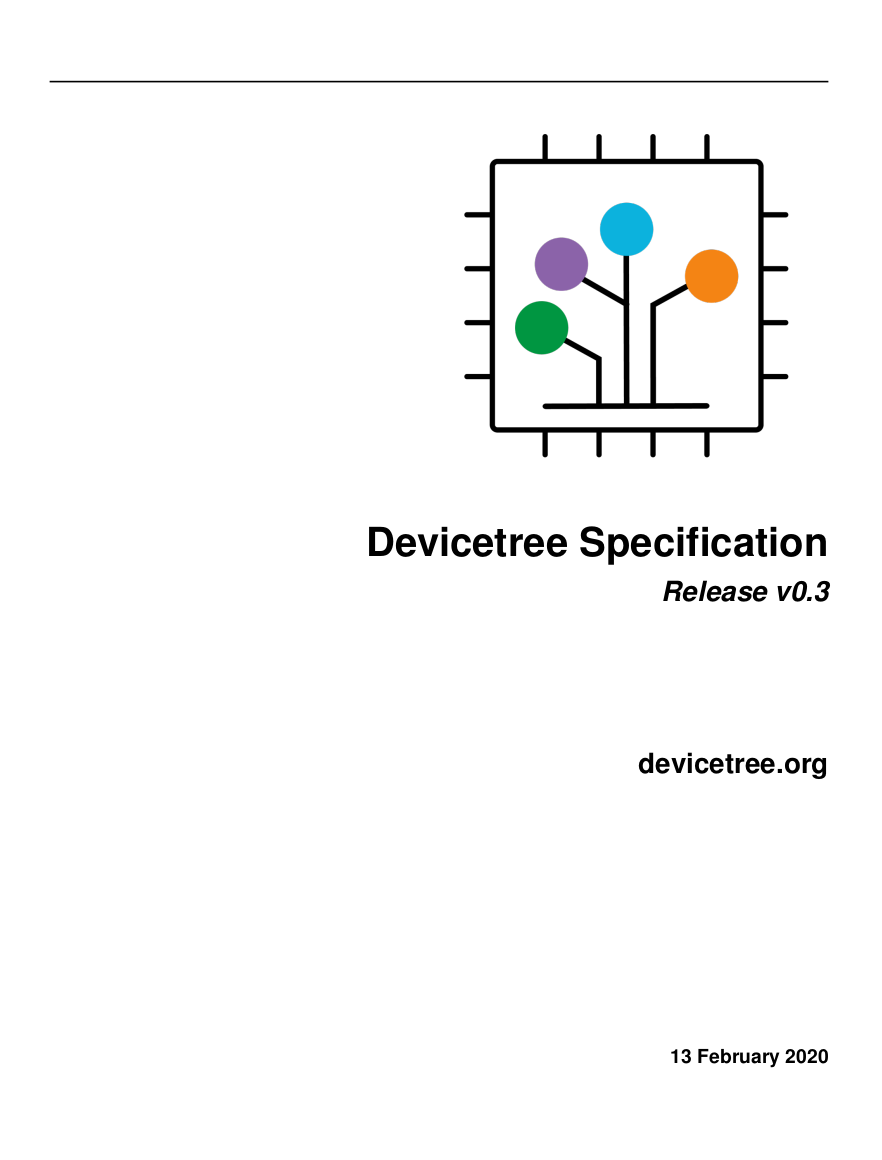
\includegraphics[width=\textwidth]{slides/sysdev-hw-devices/dt-spec.png}
  \end{columns}
\end{frame}

\begin{frame}[fragile]{Device Tree binding: old style}
  \begin{center}
    \kfile{Documentation/devicetree/bindings/mtd/spear_smi.txt}\\
    This IP is {\em not} used on STM32MP1.
  \end{center}
  \begin{columns}[t]
    \column{0.5\textwidth}
    \begin{block}{}
      {\fontsize{5}{6}\selectfont
\begin{verbatim}
* SPEAr SMI

Required properties:
- compatible : "st,spear600-smi"
- reg : Address range of the mtd chip
- #address-cells, #size-cells : Must be present if the device has sub-nodes
  representing partitions.
- interrupts: Should contain the STMMAC interrupts
- clock-rate : Functional clock rate of SMI in Hz

Optional properties:
- st,smi-fast-mode : Flash supports read in fast mode

\end{verbatim}
      }
    \end{block}
    \column{0.5\textwidth}
    \begin{block}{}
      {\fontsize{4}{5}\selectfont
\begin{verbatim}
Example:

        smi: flash@fc000000 {
                compatible = "st,spear600-smi";
                #address-cells = <1>;
                #size-cells = <1>;
                reg = <0xfc000000 0x1000>;
                interrupt-parent = <&vic1>;
                interrupts = <12>;
                clock-rate = <50000000>;        /* 50MHz */

                flash@f8000000 {
                        st,smi-fast-mode;
                        ...
                };
        };
\end{verbatim}
      }
    \end{block}
  \end{columns}

\end{frame}

\begin{frame}[fragile]{Device Tree binding: YAML style}
  \kfile{Documentation/devicetree/bindings/i2c/st,stm32-i2c.yaml}
  \begin{columns}[t]
    \column{0.5\textwidth}
    \begin{block}{}
      {\fontsize{5}{6}\selectfont
\begin{minted}{yaml}
# SPDX-License-Identifier: (GPL-2.0-only OR BSD-2-Clause)
%YAML 1.2
---
$id: http://devicetree.org/schemas/i2c/st,stm32-i2c.yaml#
$schema: http://devicetree.org/meta-schemas/core.yaml#

title: I2C controller embedded in STMicroelectronics STM32 I2C platform

maintainers:
  - Pierre-Yves MORDRET <pierre-yves.mordret@st.com>

properties:
  compatible:
    enum:
      - st,stm32f4-i2c
      - st,stm32f7-i2c
      - st,stm32mp15-i2c

  reg:
    maxItems: 1

  interrupts:
    items:
      - description: interrupt ID for I2C event
      - description: interrupt ID for I2C error

  resets:
    maxItems: 1

\end{minted}
      }
    \end{block}
    \column{0.5\textwidth}
    \begin{block}{}
      {\fontsize{5}{6}\selectfont
\begin{minted}{yaml}
  clocks:
    maxItems: 1

  dmas:
    items:
      - description: RX DMA Channel phandle
      - description: TX DMA Channel phandle

  ...

  clock-frequency:
    description: Desired I2C bus clock frequency in Hz. If not specified,
                 the default 100 kHz frequency will be used.
                 For STM32F7, STM32H7 and STM32MP1 SoCs, if timing
                 parameters match, the bus clock frequency can be from
                 1Hz to 1MHz.
    default: 100000
    minimum: 1
    maximum: 1000000

required:
  - compatible
  - reg
  - interrupts
  - resets
  - clocks
\end{minted}
      }
    \end{block}
  \end{columns}
\end{frame}

\begin{frame}[fragile]{Device Tree binding: YAML style example}
    \begin{block}{}
      {\fontsize{5}{6}\selectfont
\begin{minted}{yaml}
examples:
  - |
    //Example 3 (with st,stm32mp15-i2c compatible on stm32mp)
    #include <dt-bindings/interrupt-controller/arm-gic.h>
    #include <dt-bindings/clock/stm32mp1-clks.h>
    #include <dt-bindings/reset/stm32mp1-resets.h>
      i2c@40013000 {
          compatible = "st,stm32mp15-i2c";
          #address-cells = <1>;
          #size-cells = <0>;
          reg = <0x40013000 0x400>;
          interrupts = <GIC_SPI 33 IRQ_TYPE_LEVEL_HIGH>,
                       <GIC_SPI 34 IRQ_TYPE_LEVEL_HIGH>;
          clocks = <&rcc I2C2_K>;
          resets = <&rcc I2C2_R>;
          i2c-scl-rising-time-ns = <185>;
          i2c-scl-falling-time-ns = <20>;
          st,syscfg-fmp = <&syscfg 0x4 0x2>;
      };
\end{minted}
      }
    \end{block}
\end{frame}

\begin{frame}{Validating Device Tree in Linux}
  \begin{itemize}
  \item \code{dtc} only does syntactic validation
  \item YAML bindings allow to do semantic validation
  \item Linux kernel \code{make} rules:
    \begin{itemize}
    \item \code{make dt_binding_check}\\
      verify that YAML bindings are valid
    \item \code{make dtbs_check}\\
      validate DTs currently enabled against YAML bindings
    \item \code{make DT_SCHEMA_FILES=Documentation/devicetree/bindings/trivial-devices.yaml dtbs_check}\\
      validate DTs against a specific YAML binding
    \end{itemize}
  \end{itemize}
\end{frame}

\begin{frame}{The {\tt compatible} property}
  \begin{itemize}
  \item Is a list of strings
    \begin{itemize}
    \item From the most specific to the least specific
    \end{itemize}
  \item Describes the specific {\bf binding} to which the node complies.
  \item It uniquely identifies the {\bf programming model} of the
    device.
  \item Practically speaking, it is used by the operating system to
    find the {\bf appropriate driver} for this device.
  \item When describing real hardware, the typical form is
    \code{vendor,model}
  \item Examples:
    \begin{itemize}
    \item \code{compatible = "arm,armv7-timer";}
    \item \code{compatible = "st,stm32mp1-dwmac", "snps,dwmac-4.20a";}
    \item \code{compatible = "regulator-fixed";}
    \item \code{compatible = "gpio-keys";}
    \end{itemize}
  \item Special value: \code{simple-bus} $\rightarrow$ bus where all
    sub-nodes are memory-mapped devices
  \end{itemize}
\end{frame}

\begin{frame}{{\tt compatible} property and Linux kernel drivers}
  \begin{columns}
    \column{0.6\textwidth}
    \begin{itemize}
    \item Linux identifies as {\bf platform devices}:
      \begin{itemize}
      \item Top-level DT nodes with a \code{compatible} string
      \item Sub-nodes of \code{simple-bus}
        \begin{itemize}
        \item Instantiated automatically at boot time
        \end{itemize}
      \end{itemize}
    \item Sub-nodes of I2C controllers $\rightarrow$ {\em I2C devices}
    \item Sub-nodes of SPI controllers $\rightarrow$ {\em SPI devices}
    \item Each Linux driver has a table of compatible strings it supports
      \begin{itemize}
      \item \kstruct{of_device_id}\code{[]}
      \end{itemize}
    \item When a DT node compatible string matches a given driver, the
      device is {\em bound} to that driver.
    \end{itemize}
    \column{0.4\textwidth}
    \includegraphics[width=\textwidth]{slides/sysdev-hw-devices/dt-to-devices.pdf}
  \end{columns}
\end{frame}

\begin{frame}[fragile]{Matching with drivers in Linux: platform driver}
  \begin{block}{\kfile{drivers/tty/serial/stm32-usart.c}}
    {\tiny
\begin{minted}{c}
static const struct of_device_id stm32_match[] = {
        { .compatible = "st,stm32-uart", .data = &stm32f4_info},
        { .compatible = "st,stm32f7-uart", .data = &stm32f7_info},
        { .compatible = "st,stm32h7-uart", .data = &stm32h7_info},
        {},
};
MODULE_DEVICE_TABLE(of, stm32_match);

...

static struct platform_driver stm32_serial_driver = {
        .probe          = stm32_serial_probe,
        .remove         = stm32_serial_remove,
        .driver = {
                .name   = DRIVER_NAME,
                .pm     = &stm32_serial_pm_ops,
                .of_match_table = of_match_ptr(stm32_match),
        },
};
\end{minted}
    }
  \end{block}
\end{frame}

\begin{frame}[fragile]{Matching with drivers in Linux: I2C driver}
  \begin{block}{\kfile{sound/soc/codecs/cs42l51.c}}
    {\tiny
\begin{minted}{c}
const struct of_device_id cs42l51_of_match[] = {
        { .compatible = "cirrus,cs42l51", },
        { }
};
MODULE_DEVICE_TABLE(of, cs42l51_of_match);
\end{minted}
    }
  \end{block}
  \begin{block}{\kfile{sound/soc/codecs/cs42l51-i2c.c}}
    {\tiny
\begin{minted}{c}
static struct i2c_driver cs42l51_i2c_driver = {
        .driver = {
                .name = "cs42l51",
                .of_match_table = cs42l51_of_match,
                .pm = &cs42l51_pm_ops,
        },
        .probe = cs42l51_i2c_probe,
        .remove = cs42l51_i2c_remove,
        .id_table = cs42l51_i2c_id,
};
\end{minted}
    }
  \end{block}
\end{frame}

\begin{frame}[fragile]{{\tt reg} property}
  \begin{itemize}
  \item Most important property after \code{compatible}
  \item {\bf Memory-mapped} devices: base physical address and size of
    the memory-mapped registers. Can have several entries for multiple
    register areas.
\begin{onlyenv}<1>
\begin{block}{}
\begin{verbatim}
sai4: sai@50027000 {
    reg = <0x50027000 0x4>, <0x500273f0 0x10>;
};
\end{verbatim}
\end{block}
\end{onlyenv}
\pause
  \item {\bf I2C} devices: address of the device on the I2C bus.
\begin{onlyenv}<2>
\begin{block}{}
\begin{verbatim}
&i2c1 {
   hdmi-transmitter@39 {
      reg = <0x39>;
   };
   cs42l51: cs42l51@4a {
      reg = <0x4a>;
   };
};
\end{verbatim}
\end{block}
\end{onlyenv}
\pause
  \item {\bf SPI} devices: chip select number
\begin{onlyenv}<3>
\begin{block}{}
\begin{verbatim}
&qspi {
        flash0: mx66l51235l@0 {
                reg = <0>;
        };
        flash1: mx66l51235l@1 {
                reg = <1>;
        };
};
\end{verbatim}
\end{block}
\end{onlyenv}
\pause
\item The unit address must be the address of the first \code{reg}
  entry.
\begin{onlyenv}<4>
\begin{block}{}
\begin{verbatim}
sai4: sai@50027000 {
    reg = <0x50027000 0x4>, <0x500273f0 0x10>;
};
\end{verbatim}
\end{block}
\end{onlyenv}
  \end{itemize}
\end{frame}

\begin{frame}{Status property}
  \begin{itemize}
  \item The \code{status} property indicates if the device is really in
    use or not
    \begin{itemize}
    \item \code{okay} or \code{ok} $\rightarrow$ the device is really
      in use
    \item any other value, by convention \code{disabled} $\rightarrow$
      the device is not in use
    \end{itemize}
  \item In Linux, controls if a device is instantiated
  \item In \code{.dtsi} files describing SoCs: all devices that
    interface to the outside world have \code{status = disabled}
  \item Enabled on a per-device basis in the board \code{.dts}
  \end{itemize}
\end{frame}

\begin{frame}[fragile]{Resources: interrupts, clocks, DMA, reset lines, ...}
  \begin{columns}
  \column{0.5\textwidth}
  \begin{itemize}
  \item Common pattern for resources shared by multiple hardware
    blocks
    \begin{itemize}
    \item Interrupt lines
    \item Clock controllers
    \item DMA controllers
    \item Reset controllers
    \item ...
    \end{itemize}
  \item A Device Tree node describing the {\em controller} as a device
  \item References from other nodes that use resources provided by
    this {\em controller}
  \end{itemize}
  \column{0.5\textwidth}
\begin{block}{}
{\tiny
\begin{minted}{perl}
intc: interrupt-controller@a0021000 {
   compatible = "arm,cortex-a7-gic";
   #interrupt-cells = <3>;
   interrupt-controller;
   reg = <0xa0021000 0x1000>, <0xa0022000 0x2000>;
};

rcc: rcc@50000000 {
   compatible = "st,stm32mp1-rcc", "syscon";
   reg = <0x50000000 0x1000>;
   #clock-cells = <1>;
   #reset-cells = <1>;
};

dmamux1: dma-router@48002000 {
   compatible = "st,stm32h7-dmamux";
   reg = <0x48002000 0x1c>;
   #dma-cells = <3>;
   clocks = <&rcc DMAMUX>;
   resets = <&rcc DMAMUX_R>;
};

spi3: spi@4000c000 {
   interrupts = <GIC_SPI 51 IRQ_TYPE_LEVEL_HIGH>;
   clocks = <&rcc SPI3_K>;
   resets = <&rcc SPI3_R>;
   dmas = <&dmamux1 61 0x400 0x05>,  <&dmamux1 62 0x400 0x05>;
};
\end{minted}
}
\end{block}
\end{columns}
\end{frame}

\begin{frame}{Pin-muxing description}
  \begin{columns}
    \column{0.5\textwidth}
    \begin{itemize}
    \item Most modern SoCs, including the STM32MP1, have more features
      than they have pins to expose those features to the outside world.
    \item Pins are muxed: a given pin can be used for one function
      {\bf or} another
    \item A specific IP block in the SoC controls the muxing of pins:
      the {\bf pinmux controller}
    \item The Device Tree describes which pin configurations are
      possible, and which configurations are used by the different
      devices.
    \end{itemize}
    \column{0.5\textwidth}
    \includegraphics[width=\textwidth]{slides/sysdev-hw-devices/pin-muxing-principle.pdf}
  \end{columns}
\end{frame}

\begin{frame}[fragile]{Pin-muxing controllers on STM32MP1}
  \begin{block}{\kfile{arch/arm/boot/dts/stm32mp151.dtsi}}
{\tiny
\begin{minted}{perl}
pinctrl: pin-controller@50002000 {
        #address-cells = <1>;
        #size-cells = <1>;
        compatible = "st,stm32mp157-pinctrl";
        ...
        gpioa: gpio@50002000 { ... };
        gpiob: gpio@50003000 { ... };
        gpioc: gpio@50004000 { ... };
        gpiod: gpio@50005000 { ... };
        gpioe: gpio@50006000 { ... };
        gpiof: gpio@50007000 { ... };
        ...
};

pinctrl_z: pin-controller-z@54004000 {
        #address-cells = <1>;
        #size-cells = <1>;
        compatible = "st,stm32mp157-z-pinctrl";
        ranges = <0 0x54004000 0x400>;
        ...
        gpioz: gpio@54004000 { .... };
        ...
};
\end{minted}
}
  \end{block}
\end{frame}

\begin{frame}[fragile]{Pin-muxing configuration}
\begin{onlyenv}<1>
  \begin{block}{\kfile{arch/arm/boot/dts/stm32mp15-pinctrl.dtsi}}
{\tiny
\begin{minted}{perl}
&pinctrl {
        ...
        i2c1_pins_a: i2c1-0 {
                pins {
                        pinmux = <STM32_PINMUX('D', 12, AF5)>, /* I2C1_SCL */
                                 <STM32_PINMUX('F', 15, AF5)>; /* I2C1_SDA */
                        bias-disable;
                        drive-open-drain;
                        slew-rate = <0>;
                };
        };
        ...
        m_can1_pins_a: m-can1-0 {
                pins1 {
                        pinmux = <STM32_PINMUX('H', 13, AF9)>; /* CAN1_TX */
                        slew-rate = <1>;
                        drive-push-pull;
                        bias-disable;
                };
                pins2 {
                        pinmux = <STM32_PINMUX('I', 9, AF9)>; /* CAN1_RX */
                        bias-disable;
                };
        };
        ...
};
\end{minted}
}
  \end{block}
\end{onlyenv}
\begin{onlyenv}<2>
  \begin{center}
    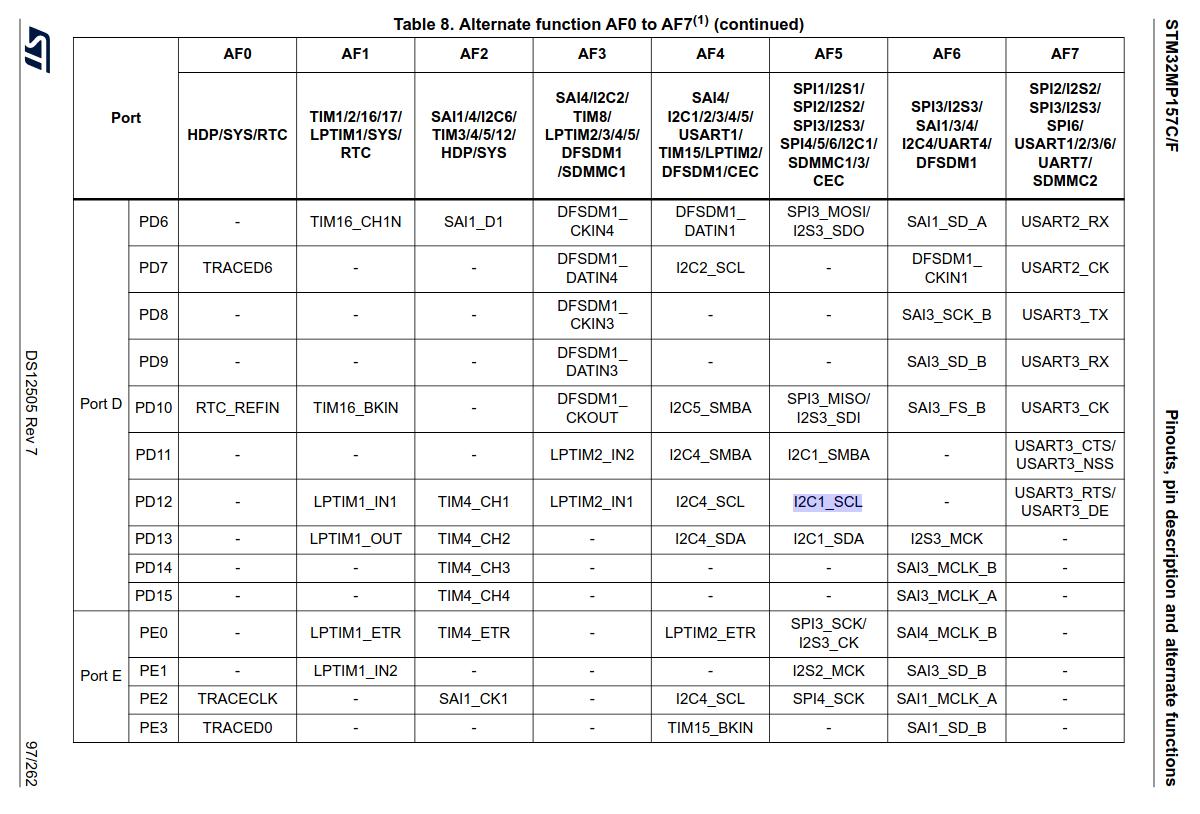
\includegraphics[height=0.78\textheight]{slides/sysdev-hw-devices/stm32mp157-i2c-pin-mux.png}
  \end{center}
  \tiny
  Source: \href{https://www.st.com/resource/en/datasheet/stm32mp157c.pdf}{STM32MP157C
  datasheet}. Note that \code{I2C1_SDA} is also available on pin \code{PF15} (not shown here).
\end{onlyenv}
\end{frame}

\begin{frame}[fragile]{Pin-muxing consumer}
  \begin{block}{}
{\tiny
\begin{minted}{perl}
&i2c1 {
        pinctrl-names = "default", "sleep";
        pinctrl-0 = <&i2c1_pins_a>;
        pinctrl-1 = <&i2c1_sleep_pins_a>;
        ...
};
\end{minted}
}
\end{block}
\begin{itemize}
\item Typically board-specific, in \code{.dts}
\item \code{pinctrl-0}, \code{pinctrl-1}, \code{pinctrl-X} provides
  the pin mux configurations for the different {\bf states}
\item \code{pinctrl-names} gives a name to each state, mandatory even
  if only one state
\item States are mutually exclusive
\item The driver is responsible for switching between states
\item \code{default} state is automatically set up when the device is
  {\em probed}
\end{itemize}
\end{frame}

\begin{frame}[fragile]{Example: LED and I2C device}
  \begin{itemize}
  \item Let's see how to describe an LED and an I2C device connected
    to the DK1 platform.
  \item Create \code{arch/arm/boot/dts/stm32mp157a-dk1-custom.dts}
    which includes \code{stm32mp157a-dk1.dts}
    \begin{block}{}
{\tiny
\begin{verbatim}
#include "stm32mp157a-dk1.dts"
\end{verbatim}
}
    \end{block}
  \item Make sure \code{stm32mp157a-dk1-custom.dts} gets compiled to a
    DTB by changing \kfile{arch/arm/boot/dts/Makefile}
    \begin{block}{}
      {\tiny
\begin{verbatim}
dtb-$(CONFIG_ARCH_STM32) += \
        ...
        stm32mp157a-dk1.dtb \
        stm32mp157a-dk1-custom.dtb \
\end{verbatim}
      }
    \end{block}
  \item \code{make dtbs}
    \begin{block}{}
      {\tiny
\begin{verbatim}
  DTC     arch/arm/boot/dts/stm32mp157a-dk1-custom.dtb
\end{verbatim}
      }
    \end{block}
  \end{itemize}
\end{frame}

\begin{frame}[fragile]{Example: describe an LED}
  \begin{columns}
    \column{0.5\textwidth}
  \begin{block}{stm32mp157a-dk1-custom.dts}
    {\tiny
\begin{minted}{perl}
#include "stm32mp157a-dk1.dts"

/ {
        leds {
                compatible = "gpio-leds";
                webinar {
                        label = "webinar";
                        gpios = <&gpioe 1 GPIO_ACTIVE_HIGH>;
                };
        };
};
\end{minted}
      }
  \end{block}
  \begin{block}{shell}
{\tiny
\begin{verbatim}
# echo 255 > /sys/class/leds/webinar/brightness
\end{verbatim}
}
\end{block}
  \column{0.5\textwidth}
  \begin{center}
    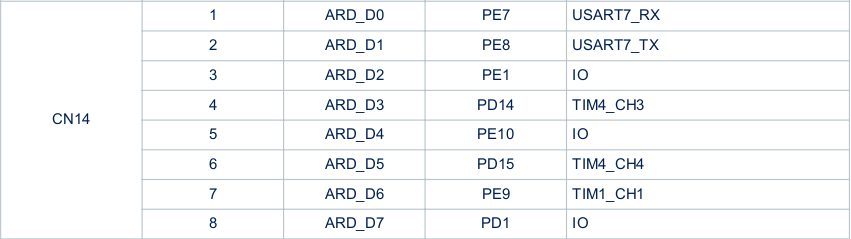
\includegraphics[height=0.3\textheight]{slides/sysdev-hw-devices/cn14-pinout.png}\\
    \vspace{0.5cm}
    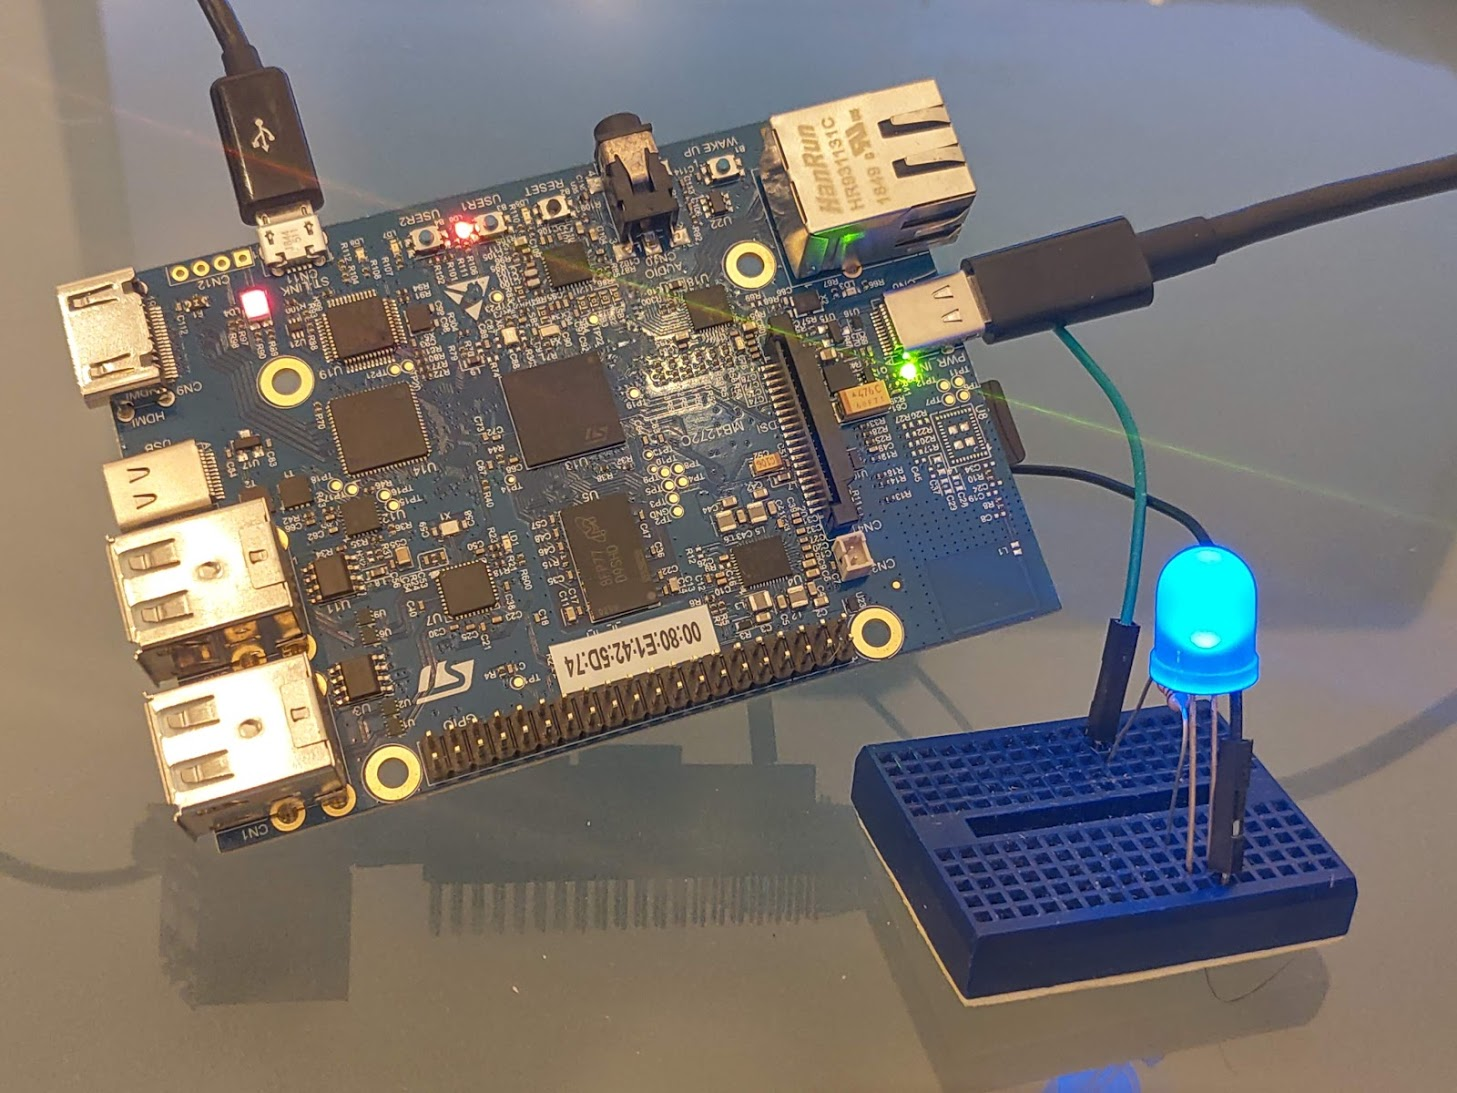
\includegraphics[height=0.3\textheight]{slides/sysdev-hw-devices/led-on.jpg}
  \end{center}
  \end{columns}
\end{frame}

\begin{frame}[fragile]{Example: connect I2C temperature, humidity and pressure sensor}
  \begin{columns}
    \column{0.5\textwidth}
    \begin{block}{stm32mp157a-dk1-custom.dts}
      {\tiny
\begin{minted}{perl}
&i2c5 {
        status = "okay";
        clock-frequency = <100000>;
        pinctrl-names = "default", "sleep";
        pinctrl-0 = <&i2c5_pins_a>;
        pinctrl-1 = <&i2c5_pins_sleep_a>;

        pressure@76 {
                compatible = "bosch,bme280";
                reg = <0x76>;
        };
};
\end{minted}
}
  \end{block}

\begin{block}{shell}
{\tiny
\begin{verbatim}
# cat /sys/bus/iio/devices/iio\:device2/in_humidityrelative_input
49147
# cat /sys/bus/iio/devices/iio\:device2/in_pressure_input
101.567167968
# cat /sys/bus/iio/devices/iio\:device2/in_temp_input
24380
\end{verbatim}
}
\end{block}
  \column{0.5\textwidth}
  \begin{center}
    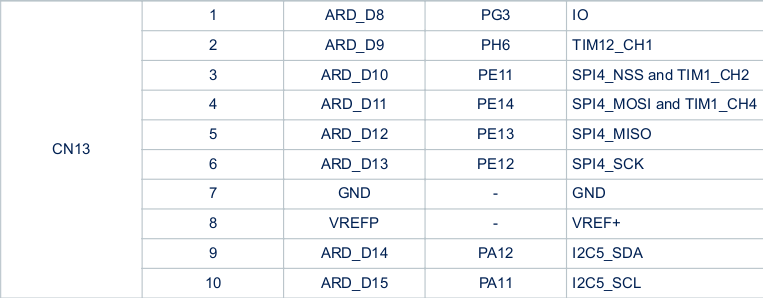
\includegraphics[width=\textwidth]{slides/sysdev-hw-devices/cn13-pinout.png}\\
    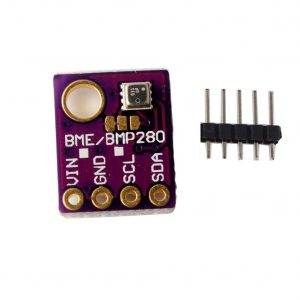
\includegraphics[width=0.4\textwidth]{slides/sysdev-hw-devices/bme.jpg}
  \end{center}
\end{columns}
\vspace{0.5cm}
Details at
\url{https://bootlin.com/blog/building-a-linux-system-for-the-stm32mp1-connecting-an-i2c-sensor/}
\end{frame}

\begin{frame}{Further details about the Device Tree}
\small
Check out our {\em Device Tree 101 webinar}, by Thomas Petazzoni (2021)
\begin{itemize}
    \item Slides: \url{https://bootlin.com/blog/device-tree-101-webinar-slides-and-videos/}\\
    \item Video: \url{https://youtu.be/a9CZ1Uk3OYQ}
\end{itemize}
\vspace{0.5cm}
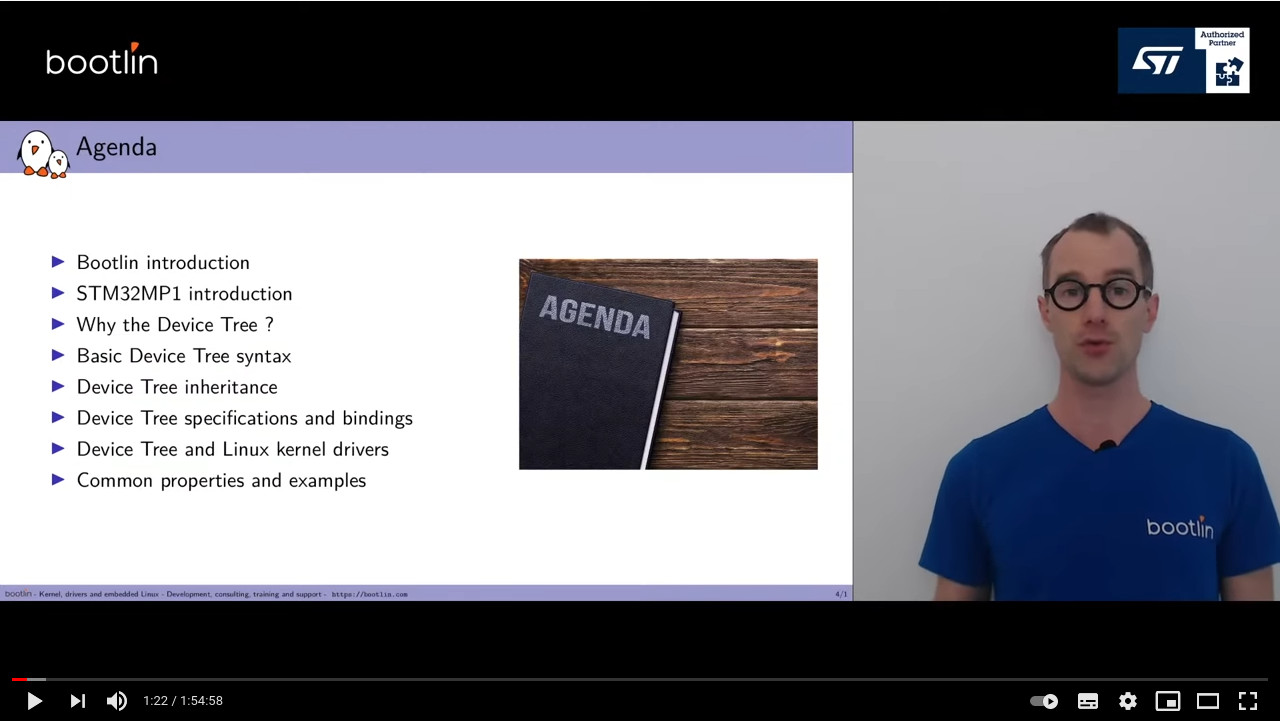
\includegraphics[height=0.5\textheight]{common/device-tree-video.jpg}
\end{frame}

\subsection{Discoverable hardware: USB and PCI}

\begin{frame}{Discoverable hardware}
  \begin{itemize}
  \item Some busses have built-in hardware discoverability mechanisms
  \item Most common busses: USB and PCI
  \item Hardware devices can be enumerated, and their characteristics
    retrieved with just a driver or the bus controller
  \item Useful Linux commands
    \begin{itemize}
    \item \code{lsusb}, lists all USB devices detected
    \item \code{lspci}, lists all PCI devices detected
    \item A detected device does not mean it has a kernel driver
      associated to it!
    \end{itemize}
  \item Association with kernel drivers done based on product
    ID/vendor ID, or some other characteristics of the device: device
    class, device sub-class, etc.
  \end{itemize}
\end{frame}

\setuplabframe
{Accessing hardware devices}
{
  Time to start the practical lab!
  \begin{itemize}
  \item Exploring the contents of \code{/dev} and \code{/sys} and the
    devices available on the embedded hardware platform.
  \item Using GPIOs and LEDs.
  \item Modifying the Device Tree to control pin multiplexing and
        declare an I2C-connected joystick.
  \item Adding support for a USB audio card using Linux kernel modules
  \item Adding support for the I2C-connected joystick through
        an out-of-tree module.
  \end{itemize}
}
